% Vehicle Counter App — User Flow
% Compile with: pdflatex flowchart.tex
% Requires: tikz, shapes.geometric, arrows.meta, positioning, fit, backgrounds
\documentclass[border=12pt]{standalone}
\usepackage{tikz}
\usetikzlibrary{
  shapes.geometric,
  arrows.meta,
  positioning,
  fit,
  backgrounds,
  calc
}

% ── Colour palette ───────────────────────────────────────────────────────────
\definecolor{mainbg}    {HTML}{E8F4FF}
\definecolor{mainborder}{HTML}{4F8EF7}
\definecolor{greenbg}   {HTML}{E8FFF2}
\definecolor{greenborder}{HTML}{30D158}
\definecolor{purplebg}  {HTML}{F5EEFF}
\definecolor{purpleborder}{HTML}{BF5AF2}
\definecolor{redbg}     {HTML}{FFF0EF}
\definecolor{redborder} {HTML}{FF453A}
\definecolor{exportbg}  {HTML}{EFFFEF}
\definecolor{darkbg}    {HTML}{1C1C1E}
\definecolor{textdark}  {HTML}{1C1C1E}
\definecolor{textsub}   {HTML}{555555}

% ── Node styles ──────────────────────────────────────────────────────────────
\tikzset{
  base/.style = {
    rectangle, rounded corners=6pt,
    minimum width=5cm, minimum height=1cm,
    text width=4.8cm, align=center,
    font=\small, inner sep=6pt,
    draw, thick
  },
  main/.style     = {base, fill=mainbg,    draw=mainborder,  text=textdark},
  green/.style    = {base, fill=greenbg,   draw=greenborder, text=textdark},
  purple/.style   = {base, fill=purplebg,  draw=purpleborder,text=textdark},
  red/.style      = {base, fill=redbg,     draw=redborder,   text=textdark},
  export/.style   = {base, fill=exportbg,  draw=greenborder, text=textdark},
  terminal/.style = {
    ellipse, fill=darkbg, text=white,
    minimum width=4cm, minimum height=0.9cm,
    font=\small\bfseries, align=center,
    draw=darkbg, thick
  },
  smallnode/.style = {
    rectangle, rounded corners=5pt,
    minimum width=3.2cm, minimum height=0.75cm,
    text width=3cm, align=center,
    font=\footnotesize, inner sep=4pt,
    draw, thick
  },
  sm-purple/.style = {smallnode, fill=purplebg, draw=purpleborder},
  sm-green/.style  = {smallnode, fill=greenbg,  draw=greenborder},
  sm-red/.style    = {smallnode, fill=redbg,     draw=redborder},
  decision/.style  = {
    diamond, aspect=2.5,
    fill=redbg, draw=redborder, thick,
    minimum width=3.5cm, minimum height=1cm,
    text width=2.8cm, align=center,
    font=\footnotesize, inner sep=3pt
  },
  arr/.style  = {-{Stealth[length=6pt]}, thick, color=textdark},
  darr/.style = {-{Stealth[length=5pt]}, thick, dashed, color=gray!60},
}

\begin{document}
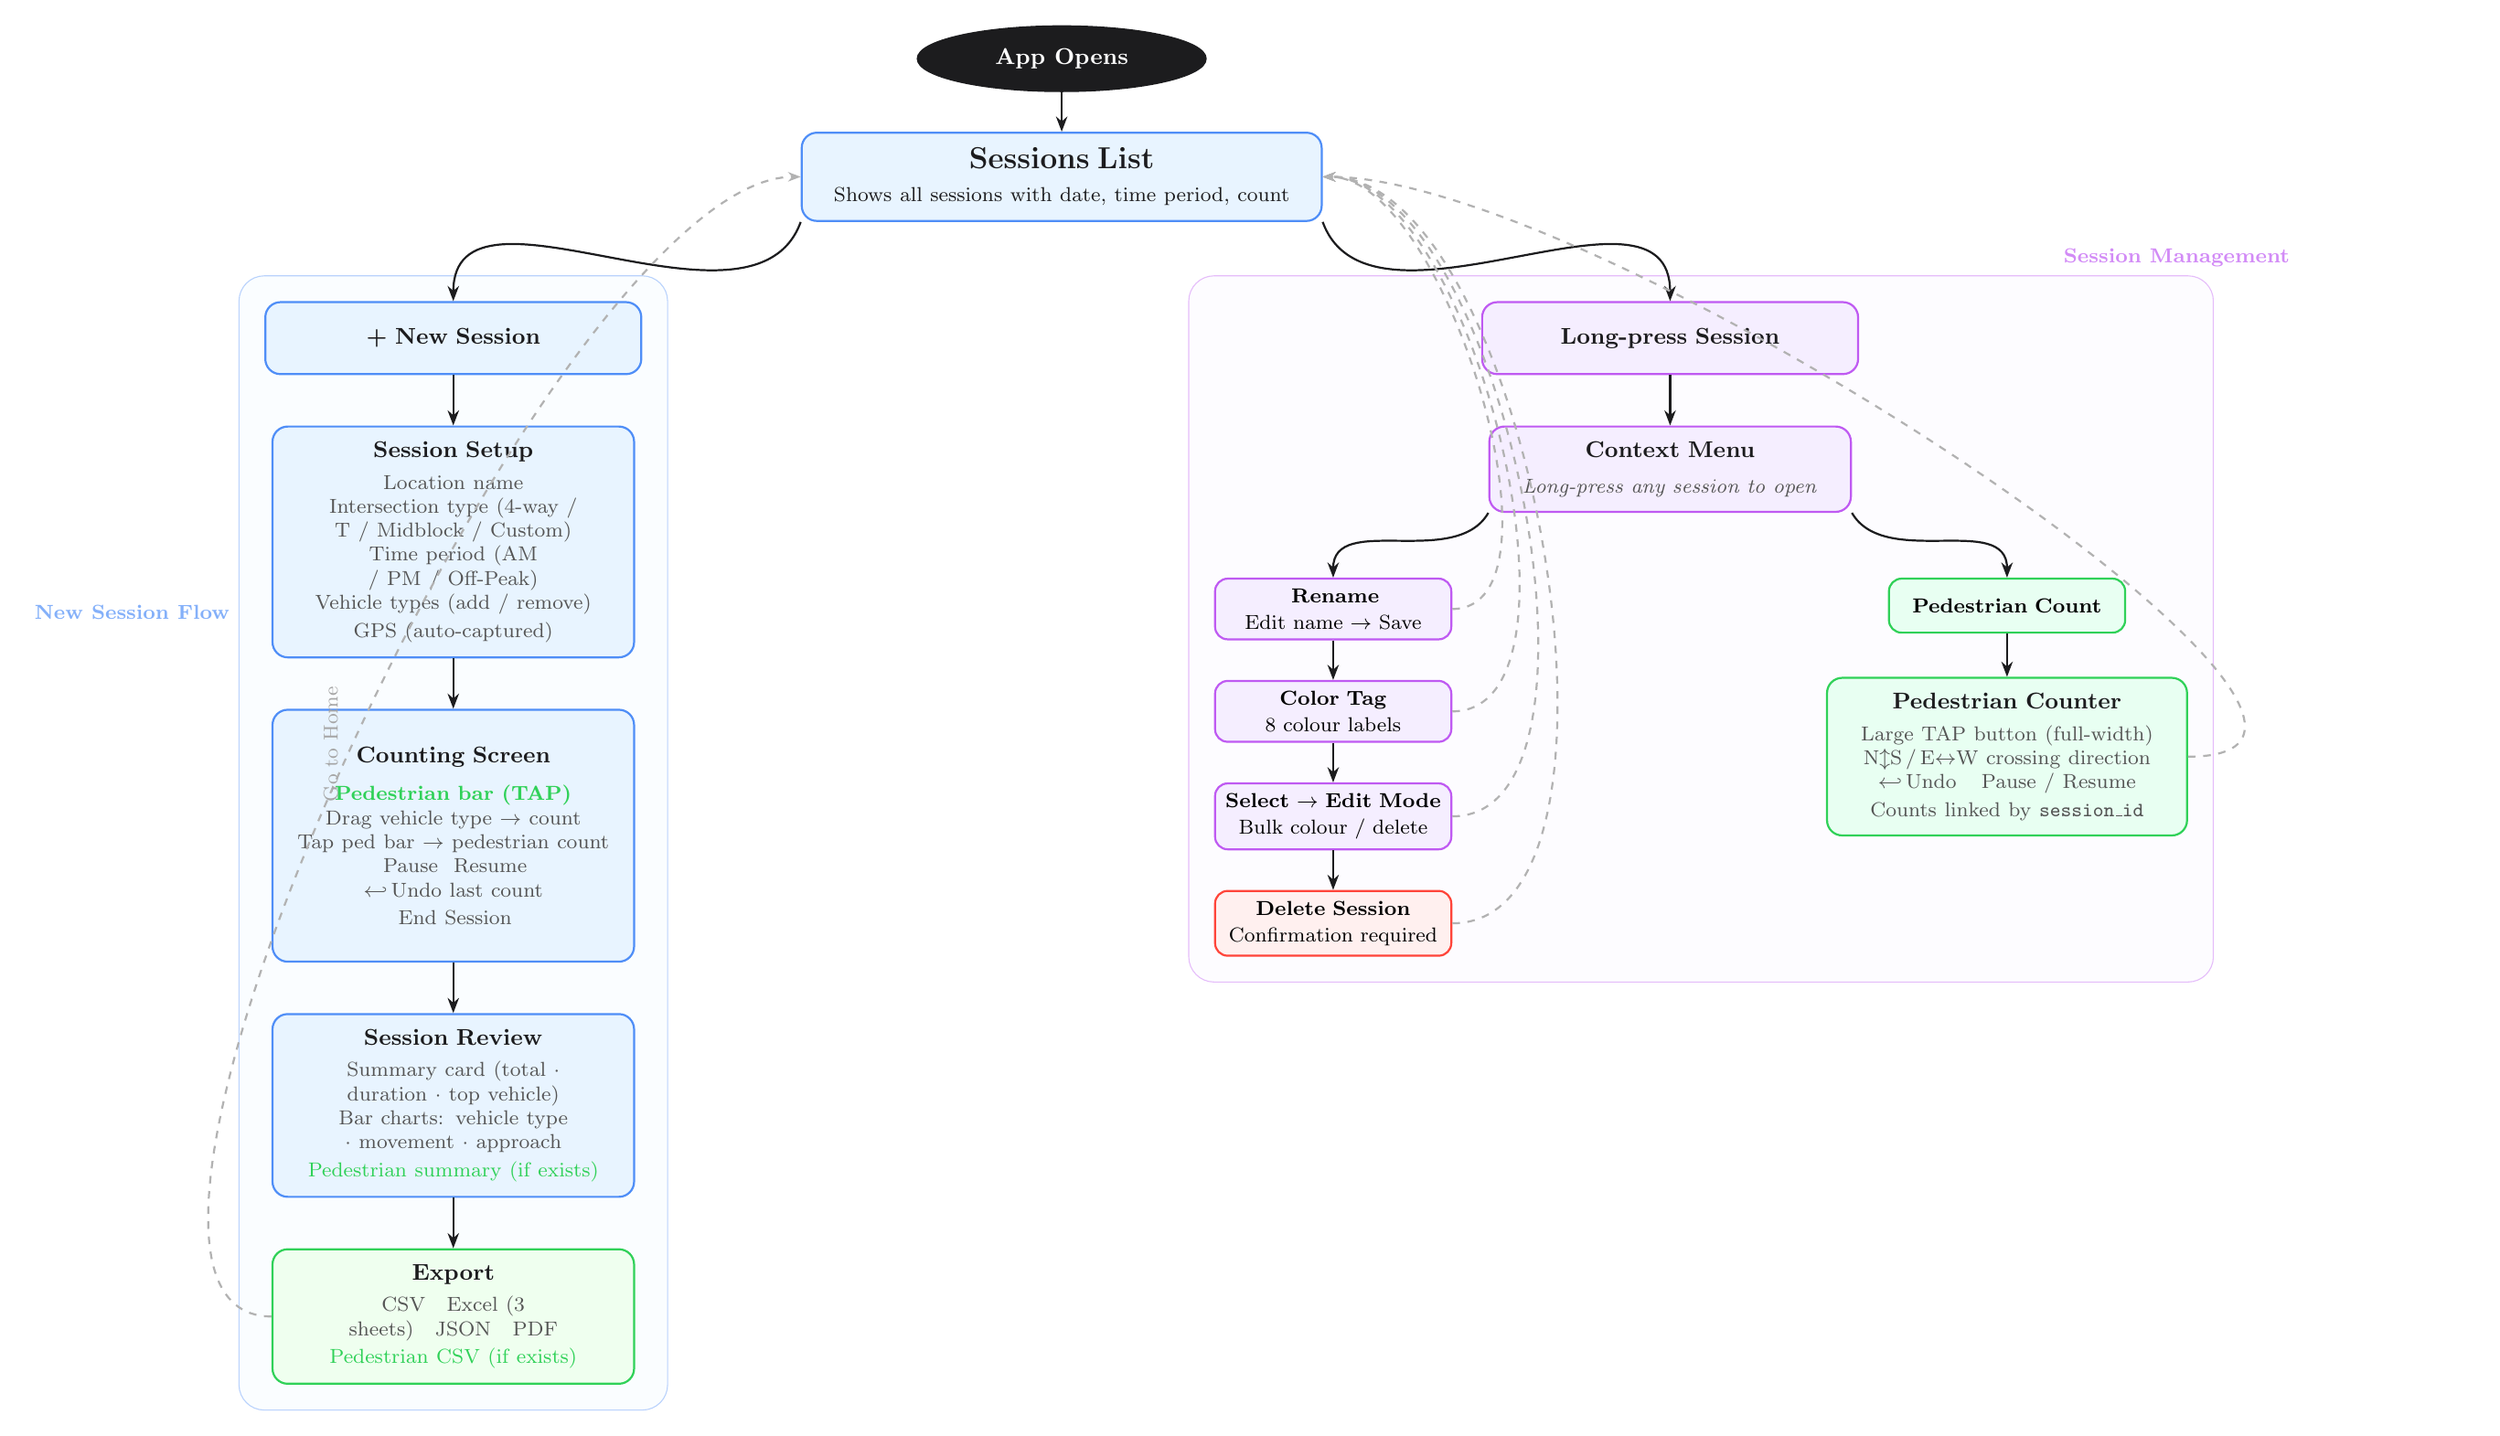
\begin{tikzpicture}[node distance=0.7cm and 1.8cm]

% ── START ───────────────────────────────────────────────────────────────────
\node[terminal] (start)
  {\textbf{App Opens}};

% ── SESSIONS LIST ───────────────────────────────────────────────────────────
\node[main, below=0.55cm of start, minimum width=7cm, text width=6.8cm] (sessions)
  {\textbf{\large Sessions List}\\[2pt]
   \footnotesize Shows all sessions with date, time period, count};

% ── LEFT BRANCH — NEW SESSION FLOW ──────────────────────────────────────────
\node[main, below left=1.1cm and 2.2cm of sessions] (newbtn)
  {\textbf{+ New Session}};

\node[main, below=0.7cm of newbtn, text width=4.6cm] (setup)
  {\textbf{Session Setup}\\[3pt]
   \footnotesize\textcolor{textsub}{%
     Location name\\
     Intersection type (4-way / T / Midblock / Custom)\\
     Time period (AM / PM / Off-Peak)\\
     Vehicle types (add / remove)\\
     GPS (auto-captured)}};

\node[main, below=0.7cm of setup, minimum height=3.5cm, text width=4.6cm] (counting)
  {\textbf{Counting Screen}\\[4pt]
   \textcolor{greenborder}{\footnotesize\textbf{Pedestrian bar (TAP)}}\\
   \footnotesize\textcolor{textsub}{%
     Drag vehicle type $\rightarrow$ count\\
     Tap ped bar $\rightarrow$ pedestrian count\\
     $\blacktriangleright$\,Pause $\diagup$ Resume\\
     $\hookleftarrow$\,Undo last count\\
     $\blacksquare$\,End Session}};

\node[main, below=0.7cm of counting, text width=4.6cm] (review)
  {\textbf{Session Review}\\[3pt]
   \footnotesize\textcolor{textsub}{%
     Summary card (total $\cdot$ duration $\cdot$ top vehicle)\\
     Bar charts: vehicle type $\cdot$ movement $\cdot$ approach\\
     \textcolor{greenborder}{Pedestrian summary (if exists)}}};

\node[export, below=0.7cm of review, text width=4.6cm] (export)
  {\textbf{Export}\\[3pt]
   \footnotesize\textcolor{textsub}{%
     CSV\quad Excel (3 sheets)\quad JSON\quad PDF\\
     \textcolor{greenborder}{Pedestrian CSV (if exists)}}};

% ── RIGHT BRANCH — SESSION MANAGEMENT ───────────────────────────────────────
\node[purple, below right=1.1cm and 2.2cm of sessions] (longpress)
  {\textbf{Long-press Session}};

\node[purple, below=0.7cm of longpress, text width=4.6cm] (context)
  {\textbf{Context Menu}\\[3pt]
   \footnotesize\textcolor{textsub}{%
     \textit{Long-press any session to open}}};

% Context menu options
\node[sm-purple, below left=0.9cm and 0.5cm of context] (rename)
  {\textbf{$\checkmark$\,Rename}\\[1pt]\footnotesize Edit name $\rightarrow$ Save};

\node[sm-purple, below=0.55cm of rename] (coloropt)
  {\textbf{Color Tag}\\[1pt]\footnotesize 8 colour labels};

\node[sm-purple, below=0.55cm of coloropt] (selectopt)
  {\textbf{Select $\rightarrow$ Edit Mode}\\[1pt]\footnotesize Bulk colour / delete};

\node[sm-green, below right=0.9cm and 0.5cm of context] (pedopt)
  {\textbf{Pedestrian Count}};

\node[green, below=0.6cm of pedopt, text width=4.4cm] (pedscreen)
  {\textbf{Pedestrian Counter}\\[3pt]
   \footnotesize\textcolor{textsub}{%
     Large TAP button (full-width)\\
     N$\updownarrow$S\,/\,E$\leftrightarrow$W crossing direction\\
     $\hookleftarrow$\,Undo\quad $\blacktriangleright$\,Pause / Resume\\
     Counts linked by \texttt{session\_id}}};

\node[sm-red, below=0.55cm of selectopt] (deleteopt)
  {\textbf{Delete Session}\\[1pt]\footnotesize Confirmation required};

% ── ARROWS — LEFT BRANCH ────────────────────────────────────────────────────
\draw[arr] (start)    -- (sessions);
\draw[arr] (sessions.south west) to[out=250,in=90]  (newbtn.north);
\draw[arr] (newbtn)   -- (setup);
\draw[arr] (setup)    -- (counting);
\draw[arr] (counting) -- (review);
\draw[arr] (review)   -- (export);

% Go to Home — curved back up left side
\draw[darr] (export.west)
  to[out=180, in=180, looseness=0.5]
  node[midway, left=2pt, font=\footnotesize, text=gray!70]
    {\rotatebox{90}{\hspace*{2pt}Go to Home}}
  (sessions.west);

% ── ARROWS — RIGHT BRANCH ───────────────────────────────────────────────────
\draw[arr] (sessions.south east) to[out=290,in=90] (longpress.north);
\draw[arr] (longpress) -- (context);
\draw[arr] (context.south west) to[out=240,in=90] (rename.north);
\draw[arr] (rename)    -- (coloropt);
\draw[arr] (coloropt)  -- (selectopt);
\draw[arr] (selectopt) -- (deleteopt);
\draw[arr] (context.south east) to[out=300,in=90] (pedopt.north);
\draw[arr] (pedopt)    -- (pedscreen);

% Return arrows → Sessions List (right side curved)
\foreach \nd in {rename, coloropt, selectopt, deleteopt, pedscreen} {
  \draw[darr] (\nd.east) to[out=0, in=0, looseness=0.7] (sessions.east);
}

% ── BACKGROUNDS / SUBGRAPH LABELS ───────────────────────────────────────────
\begin{pgfonlayer}{background}

  % New Session flow group
  \node[draw=mainborder!40, fill=mainbg!20, rounded corners=10pt,
        fit=(newbtn)(setup)(counting)(review)(export),
        label={[font=\footnotesize\bfseries, text=mainborder!70]above left:New Session Flow},
        inner sep=10pt] {};

  % Management flow group
  \node[draw=purpleborder!40, fill=purplebg!20, rounded corners=10pt,
        fit=(longpress)(context)(rename)(coloropt)(selectopt)(deleteopt)(pedopt)(pedscreen),
        label={[font=\footnotesize\bfseries, text=purpleborder!70]above right:Session Management},
        inner sep=10pt] {};

\end{pgfonlayer}

\end{tikzpicture}
\end{document}
